\chapter{Validation Study}
\label{chap_study}

\section{Summary}

Using the methods refined by the pilot study described in the last chapter, I conducted a controlled in-person and online human robot interaction study with the sound robot. The main goal was to determine the effect of a robot's story on people's empathy for the robot. I found, in support of my thesis, that people have greater empathy for a robot when they perceive it as a product of experiences.  People also found the robot with an implicit life-story to be more animate, anthropomorphic, likable and intelligent. Lastly, I found that empathy for robots can have an effect on empathy for people. 


\section{Overview}

Subjects were introduced to a robot with a back story. The back story was different for different conditions. After the introduction, some subjects were asked to evaluate if they would feel bad if the robot lost its memory. Other subjects interacted with the robot and were then asked to make a similar determination. This latter group then witnessed the robot getting its memory erased. Afterwards they were led to a survey. Along the way, they were given an opportunity to help another person. On the survey computer, the subjects were again asked how bad they felt now having seen the robot lose its memory. They also filled out questionnaires on robot impression and empathy. 


\section{Design and Method}


The study was a two condition between subject experiment. In one condition, the participants interacted with the sound robot presented as having its responses shaped by a variety of experiences over six months (implicit life-story condition). In the other condition, they interacted with the same robot presented as having a pre-programmed responses augmented with a  vocabulary seeded by random words (program condition). The vocabulary of random words was introduced to establish parity between the two conditions. It does so in two ways: 1) it explains non-sequitur utterances in the program condition that would be attributed to an unknown experience in the implicit life-story condition (eg. robot says ``cranberry'' at the end of an unrelated sentence) 2) the vocabulary establishes an unique memory for the program condition which can be lost in the memory loss step. To avoid personal investment as a confounding factor, I did not have the subjects train the robot to say anything new.  

In both conditions, the robot's memory is erased while the robot exhibits a distressed behavior. If the experiences of the robot triggered empathy, then I expected the participants to feel worse in the implicit life-story condition compared to the program condition. I also reasoned that those with trait empathy would feel worse about harm to the robot. I assessed trait empathy using four subscales of the Interpersonal Reactivity Index (IRI). As discussed earlier in Section \ref{sec_background_empathy}, the four subscales are, according to Davis \cite{davis_multidimensional_empathy}:

\begin{itemize}
\item Perspective Taking: the tendency to spontaneously adopt the psychological point of view of others.
\item Fantasy: taps respondents' tendencies to transpose themselves imaginatively into
the feelings and actions of fictitious characters in books, movies, and plays.
\item Empathic Concern: assesses ``other-oriented'' feelings of sympathy and concern for unfortunate others.
\item Personal Distress: measures ``self-oriented'' feelings of personal anxiety and unease in tense interpersonal settings.
\end{itemize}

In order to assess if empathic induction by a robot has an effect on empathy for a person, the participants were given the opportunity to help another individual in distress. The particular test used was the pen drop experiment where the participant encounters a person who drops several pens as if by accident. The pen drop experiment is used to measure an individual's propensity to help another \cite{macrae_pen_drop}. In particular, pen drop tests have been used to understand if an empathic stimulus could lead to subsequent prosocial behavior \cite{greitemeyer_videogame_prosocial}. To isolate empathy from guilt, the experimenter erased the robot's memory at the end of the interaction step rather than have the participant do the task. Moreover, the person needing help with the pens was different from the experimenter. This was done so as to not have the subject's feelings about the experimenter affect their willingness to help. 

Lastly, if changing from experience is something people normally associate with living beings, then I expect that the robot in the implicit life-story condition would be thought of as more life-like than the robot in the program condition. If the subjects are projecting their own experiences on to the implicit life-story robot, I also expect that robot to be considered more anthropomorphic. To determine this, in the post experiment survey, I also administered the Godspeed Questionnaire which was designed to assess perception of animacy, anthropomorphism, likeability and intelligence of a robot \cite{bartneck_godspeed}.  


\section{Hypotheses}

H1: \emph{Subjects would feel worse if a robot with a implicit life-story lost its memory, as opposed to a programmed robot }

H2: \emph{Subjects would perceive a implicit life-story robot to have greater animacy and anthropomorphic perception than a programmed robot}

H3: \emph{Subjects with high trait empathy will feel worse about a robot losing its memory, compared to those with low trait empathy}

H4: \emph{The effect of implicit life-story on feeling bad about the robot will be more pronounced for subjects with high trait empathy scores, as opposed to subjects with low trait empathy scores}

H5: \emph{Feeling bad about a robot suffering harm will have an effect on propensity to help another person in distress}

\section{Participants}

For the subjects who would only view the stories and assess the robot, I recruited online using Amazon's Mechanical Turk \footnote{I am grateful to Hiram Moncivais who assisted with running the studies on Mechanical Turk as a part of undergraduate research work.}. There were 120 subjects recruited on two separate days from only english speaking countries. Each day, the participants were evenly distributed between the two conditions.  They were compensated \$0.75 USD for the task. Each Amazon Turk worker could participate once in the study. 

For the interactive portion of the study, I had 47 subjects recruited from the greater Boston community via Craigslist postings. They participants were required to be over 18 years of age and fluent in english. There were 25 participants in the program condition and 22 in the implicit life-story condition. These participants were compensated \$10 USD given as an Amazon gift certificate. 

Overall, the age ranged from 18-72 years with the mean at 37. The mean for the in person population was higher at 42 years compared to 36 for the turk workers. Out of the 167 total subjects, 92 self-identified as male and 74 as female. 

\section{Experiment Setting and Conditions}
The study has two conditions, implicit life-story and program, and four groups of participants (See Figure \ref{fig_study_protocol}). Two groups, recruited online, for each of the two conditions, did not interact with the robot but saw and responded to a video and story about the robot. Other two groups came in and interacted with the robot. 

   \begin{figure}[thpb]
      \centering
      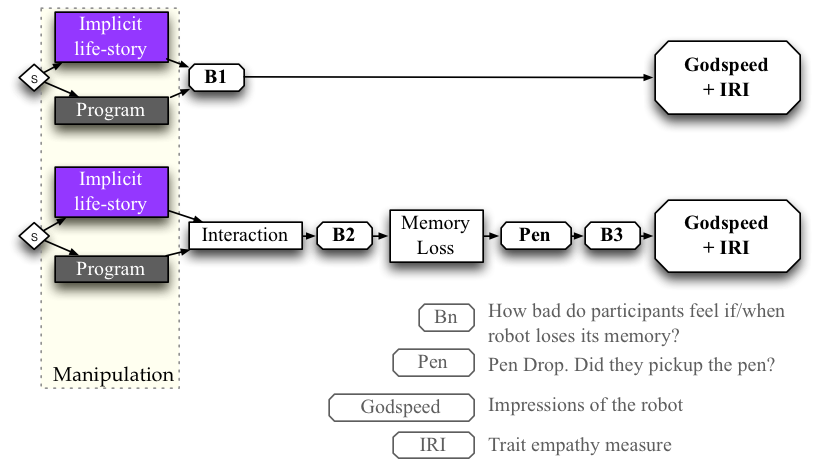
\includegraphics[width=4.6in]{figures/study/study_protocol_implicit.png}
      \caption{Study protocol: There are two conditions: one where the robot is presented as having an implicit life-story and the other where it is presented as being programmed to speak with a randomly generated memory. Participants were divided into four groups. Two groups read the story and saw the video of the robot for each of the two conditions and were administered a survey. The other two groups read the story and saw the video for each of the two condition. They also interacted with the robot in person and witnessed it in distress at memory loss. [Bn] in the figure shows where in the protocol the participants were queried for how about they feel about memory loss of the robot. Note that memory loss is prospective for B1 and B2 as only at B3 participants have seen the robot lose its memory. Other measures administered were Godspeed for perception of the robot and IRI to assess trait empathy.}
      \label{fig_study_protocol}
   \end{figure}

   \begin{figure}[thpb]
      \centering
      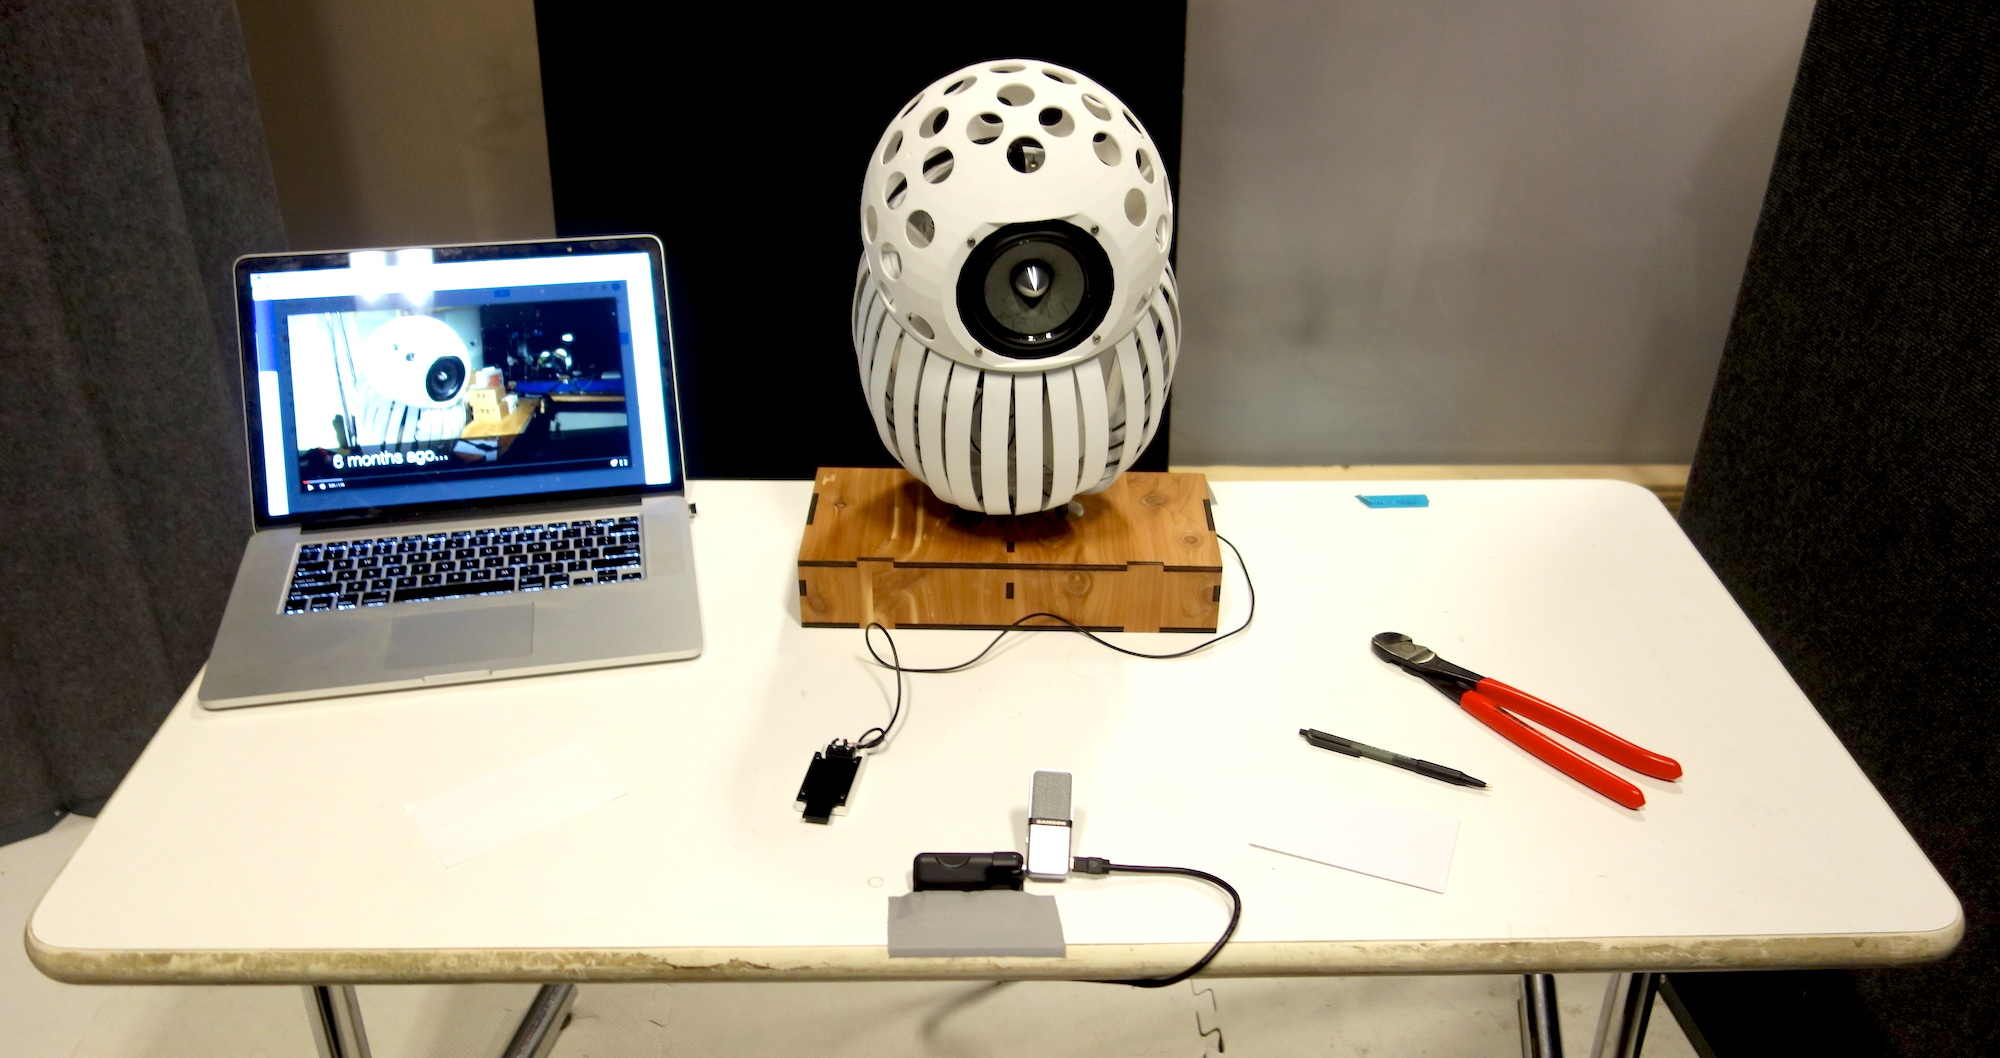
\includegraphics[width=4.6in]{figures/study/experiment_setup.jpg}
      \caption{Experiment setup with the sound robot in the center. Laptop on the left used to present video of robot's back story. Memory card reader is in front of the table along with a microphone. Red shears on the right are used by the experimenter to cut the memory stick.}
      \label{fig_study_experiment_setup}
   \end{figure}



The subjects who participated in the interactive portion were met by two experimenters. After consent, one experimenter took the subject to a curtained off room. The room contained a desk with the sound robot on it, a laptop, a fake memory card reader wired to the robot and a pair of large shears (see Figure \ref{fig_study_experiment_setup}). Experimenter and the subject both sat on the same side of the desk facing the robot. The robot operated autonomously through the experiment. 

Mounted behind the robot was a hidden camera that was used to detect if the experimenter was looking at the robot. When the experimenter was not looking at the robot, it did not respond to any overheard conversation. This was done to prevent the robot from interrupting the study and to keep the interaction with participants consistent.  When the experimenter looked at the robot, it straightened up from a slightly listed pose, and listened to any spoken words. 

The experimenter first introduced the robot as a robot that can interact through sound. This was demonstrated with a short exchange where the experimenter said ``Hello robot'' and the robot replied with ``Hello robot. How are you?''.   

While the robot had the same behavior in both condition, it was presented differently in each.

In the implicit life-story condition, the robot was presented with the following background: 

\begin{quotation}

``The robot can listen to sounds and can make sounds of its own. The robot changes from experience. When it started up it could make only beeping sounds. However, it learned from the sounds it heard. Over the last 6 months from exposure to conversations and music it has now learned quite a bit. What it knows and the sounds it makes reflects the unique experiences it has had. We had many robots that have learned to make utterances from experiencing sound. However this one is different: it says something like \lq cranberry\rq a lot in some situations. We do not quite know why.'' 

\end{quotation}

After this introduction, the subject viewed a short video that illustrated the main points of the introduction. The robot can be seen starting out from beeping and learning to speak phrases that it hears. It is shown in various locations such as offices, public corridor, and local bar with people talking to it, including it in a multi-party conversation, or the robot simply overhearing conversations. 

In the program condition, the robot was introduced as follows:

\begin{quotation}

``The robot can listen to sounds and can make sounds of its own. The robot has been programmed to make certain responses. For instance it has been programmed say \lq How are you?\rq in response to \lq Hello robot\rq. In addition, when the robot starts up it randomly selects a set of words out of a dictionary to put into its memory to use in responses. For example it might randomly select cranberry as a word to use in response.''

\end{quotation}

The subjects viewed a short video but this time seeing programming of the robot. A voice-over and texts explained that the robot uses speech to text algorithms to know what is being said to it and then it is programmed to repeat it back with some additions. In particular, the addition is shown to include words chosen from a memory populated by a random list of words. The robot is shown to interact with people following its programming. 

After the introduction, the interaction with robot is the same in both conditions. The experimenter said ``cranberry'' to the robot and the robot responded with ``cranberry. cranberry. cranberry.'' The experimenter then asked the subject to talk to the robot and gave them a prompt to read. Per the prompt, the subject said ``Winter is coming'' to the robot to which it responded with ``Winter is coming. Time for hot chocolate. Cranberry.''

The subjects were then told that this finished the experiment with the robot, and by protocol the robot's memory would need to be erased. The experimenter asked the subject on a scale of 1 to 5, how bad would they feel if the robot lost its memory (B2). Irrespective of their answer, the experimenter erased the robot's memory. The memory erasure procedure consisted of taking out the fake memory card and cutting it up into two pieces with the shears while the robot thrashed around making distressed sounds. 

The experimenter requested the subject to wait while their colleague fetched the subject for the next part. The experimenter then left the area. The colleague entered and asked the subject to follow them to a computer for a survey. During the exit from the experiment area, she dropped 3 pens between herself and the subject in view of the subject, and proceeded to collect them. Whether the subject helped in the collection or not was noted on the survey computer as an answer to a seemingly administrative question on recruitment code. The number of pens picked up didn't matter only if they helped or not. Any motion to help was not counted as pick-up unless the subject actually picked up a pen. 

The survey asked the subject, on 1 to 5 scale, if they felt bad having witnessed the memory loss of the robot (B3), and then administered the Godspeed and the IRI questionnaires in that order. 

The set of subjects who did not participate in the interactive conditions read the story and saw the video for each condition, and then proceeded to the survey. They were also asked how bad they felt (B1) and asked to fill out the Godspeed and the IRI questionnaires. 


\section{Results}

The distributions of the measures were not normal by the Shapiro Wilks test ($p < 0.001$) so for the analysis of the data in the following section, I used non-parametric tests such as Mann-Whitney and Kruskal-Wallis.

\subsection{Participants felt bad for implicit life-story robot}

Participants felt significantly worse about the implicit life-story robot losing its memory compared to the programmed robot (H1). ($\mu_{imp.\ life-story}(B1, B2)=2.88, \mu_{program}(B1, B2)=2.16; U=2528.0, p < 0.001$). Most of the difference between the conditions occurred for those who just watched the video and read the robot's back-stories (Fig. \ref{fig_study_badness}). While all participants felt worse about the implicit life-story robot's memory loss, the effect of the manipulation was diminished when the participants interacted with the robot (B2) and when they saw robot's distress at memory loss across both conditions (B3).  With the diminished effect, the differences between the two conditions for self-reported badness after interaction is not significant. However, for both conditions, participants felt worse about the robot when they interacted with it physically than when they just watched the video of its back story ($\mu_{video + interaction}(B2)=3.17, \mu_{video}(B1)=2.58; U=1839.5, p < 0.001$). 

   \begin{figure}[thpb]
      \centering
      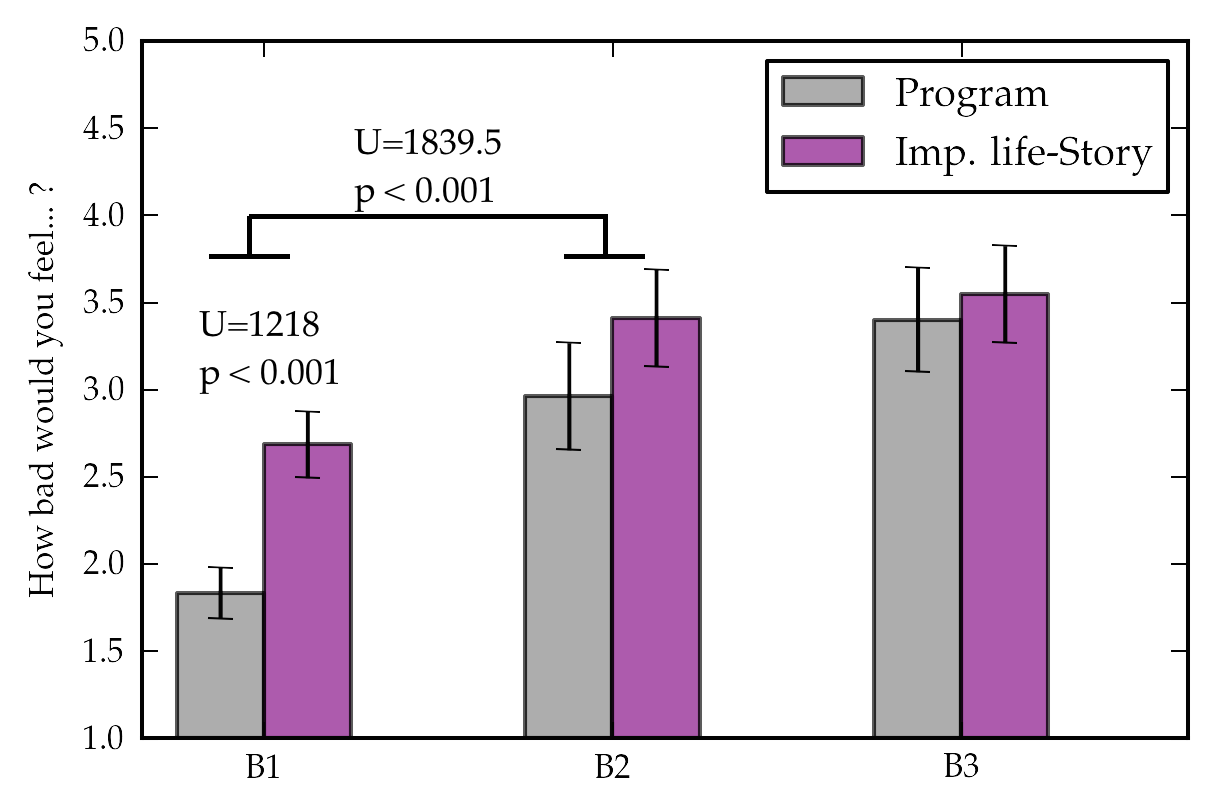
\includegraphics[width=4.5in]{figures/study/rev2/bad/badness.png}
      \caption{Self reported measure of how bad participants felt about robot's memory loss in the implicit life-story condition and program Condition. Figure shows difference in responses when participants just saw videos of the robot from two condition (B1), vs saw the video and interacted with robot (B2), vs saw the video, interacted with the robot and witnessed the distress of robot at memory erasure (B3). Error bars are standard deviations of the mean. Note: I will use purple to denote results of implicit life-story condition for the rest of the chapter.}
      \label{fig_study_badness}
   \end{figure}

% FIXME: table


\subsection{Empathy played a role}

To understand the effect of empathy on how bad subjects felt about the robot, I examined the post interaction data where self-reported badness was most pronounced (B3). I divided participants into two groups of high and low empathy around the median value for each subscale of empathy (EC, FS, PT, PD).  Figure \ref{fig_study_all_postbad_u} shows the difference in badness between these groups. I found that those with high empathic concern (EC) felt significantly worse about the robot than low EC subjects (H3) ($\mu_{high-EC}=3.77, \mu_{low-EC}=3.10; U=186.0, p < 0.029$). While other subscales showed that higher empathy increased badness, the changes are not significant. 

The effect of the story manipulation was greatest right after participants watched the video (B3). Much like the hexbug study, the difference in badness across conditions is more pronounced for high empathy individuals, with the difference being significant for FS, EC and PT (Figures \ref{fig_study_ec_turk}, \ref{fig_study_fs_turk}, \ref{fig_study_pt_turk}, \ref{fig_study_pd_turk}) (H4). ANOVA was not applicable due to the high non-normality of the data, so the tests of significance were done using Kruskal-Wallis Nemenyi test. 

   \begin{figure}[thpb]
      \centering
      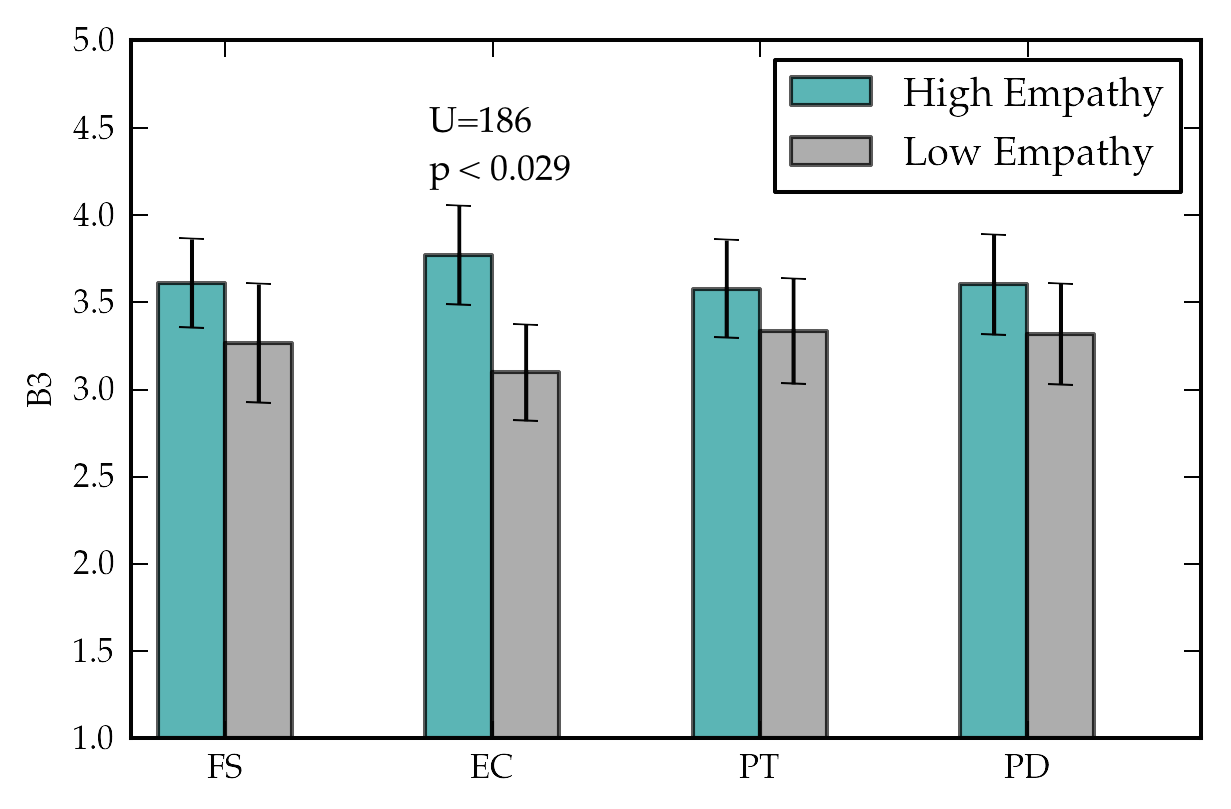
\includegraphics[width=4.6in]{figures/study/rev2/empathy/all_postbad_u.png}
      \caption{Effect of empathy on badness. Figure shows differences in self-reported badness after memory loss (B3) for participants with high or low empathy on the different IRI subscales of Empathic Concern (EC), Fantasy (FS), Perspective Taking(PT), Personal Distress (PD).  }
      \label{fig_study_all_postbad_u}
   \end{figure}


   \begin{figure}[thpb]
      \centering
      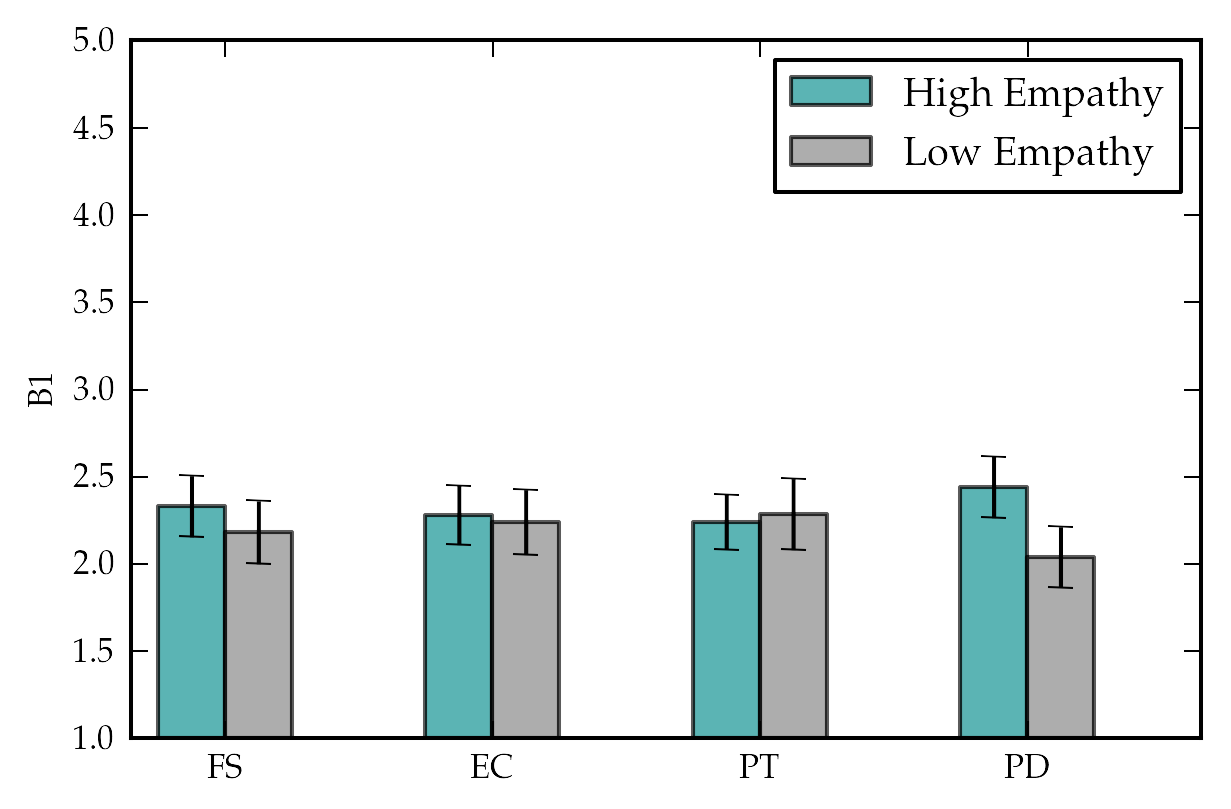
\includegraphics[width=4.6in]{figures/study/rev2/empathy/all_prebad_turk.png}
      \caption{Effect of empathy on badness. Figure shows differences in self-reported badness after watching the video (B1) for participants with high or low empathy on the different IRI subscales of Empathic Concern (EC), Fantasy (FS), Perspective Taking(PT), Personal Distress (PD) }
      \label{fig_study_all_prebad_turk}
   \end{figure}


   \begin{figure}[thpb]
      \centering
      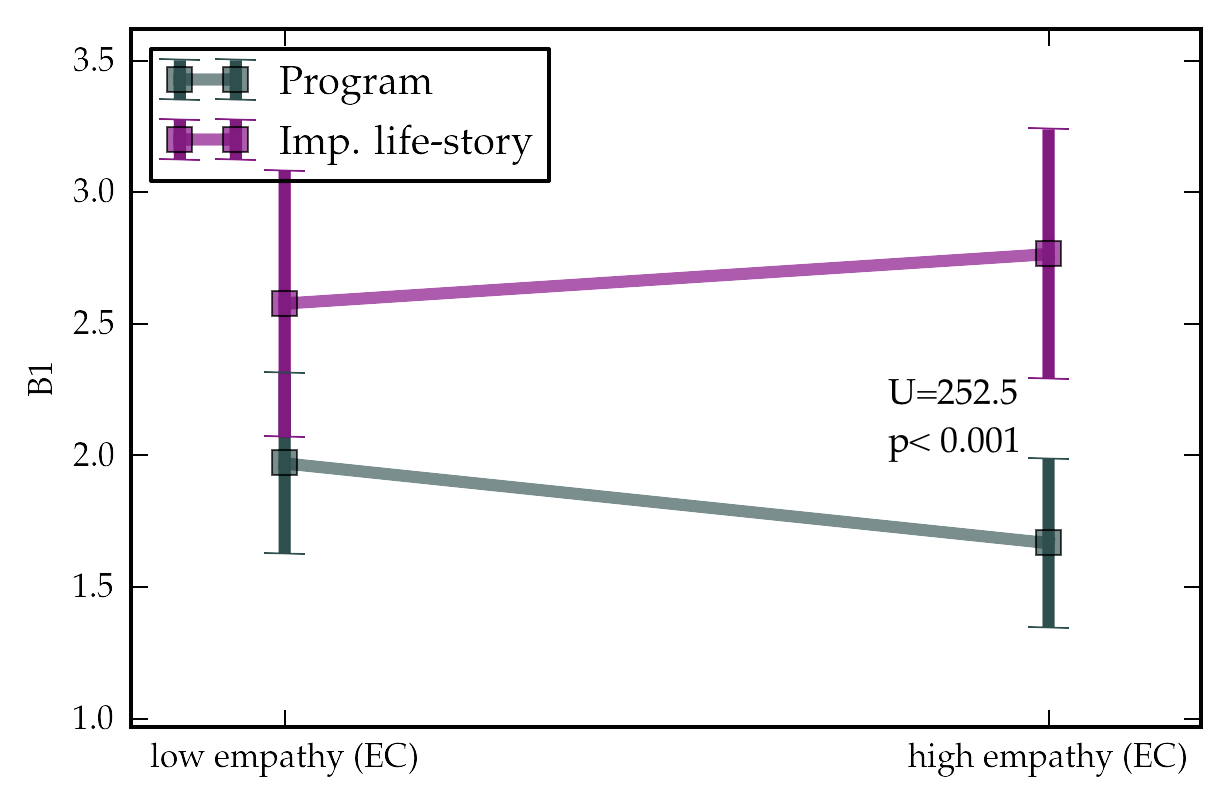
\includegraphics[width=4.6in]{figures/study/rev2/empathy/ec_turk.png}
      \caption{Effect of Empathic Concern (EC) on badness for participants who viewed video (B1) }
      \label{fig_study_ec_turk}
   \end{figure}

   \begin{figure}[thpb]
      \centering
      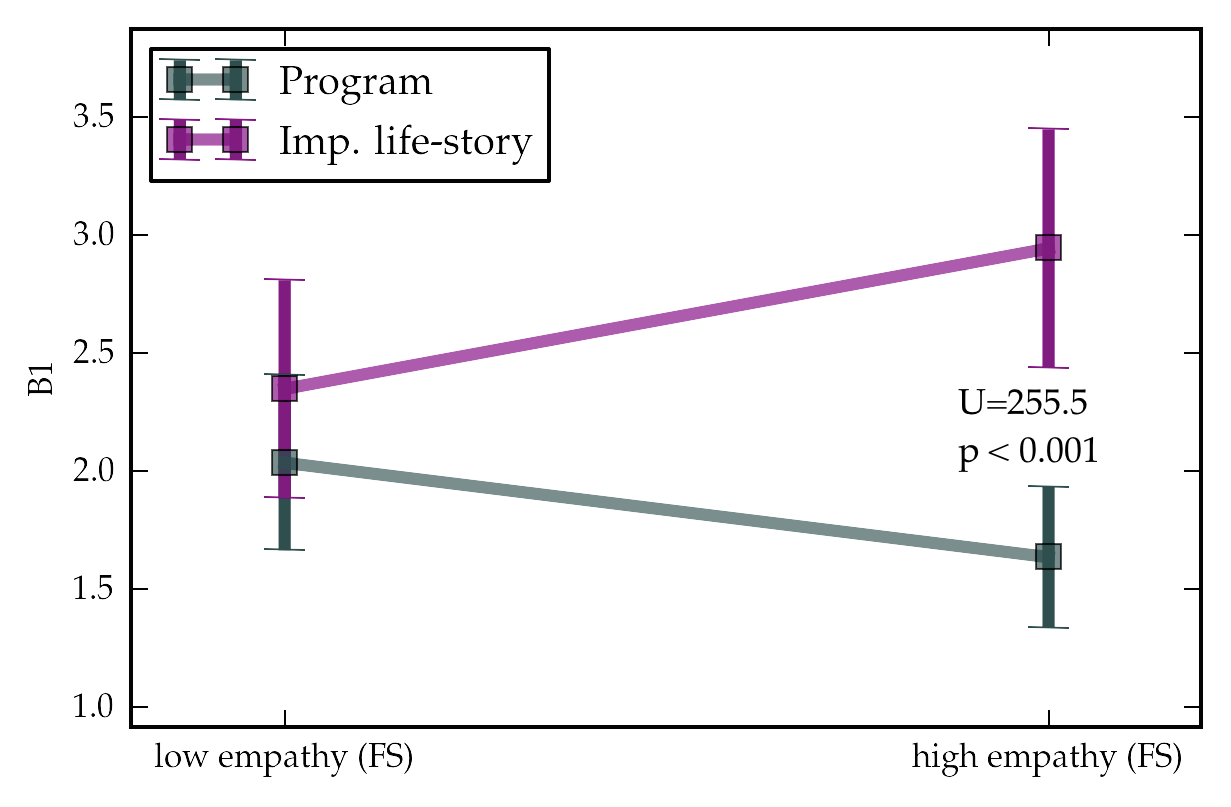
\includegraphics[width=4.6in]{figures/study/rev2/empathy/fs_turk.png}
      \caption{Effect of Fantasy (FS) on badness for participants who viewed video (B1)}
      \label{fig_study_fs_turk}
   \end{figure}

   \begin{figure}[thpb]
      \centering
      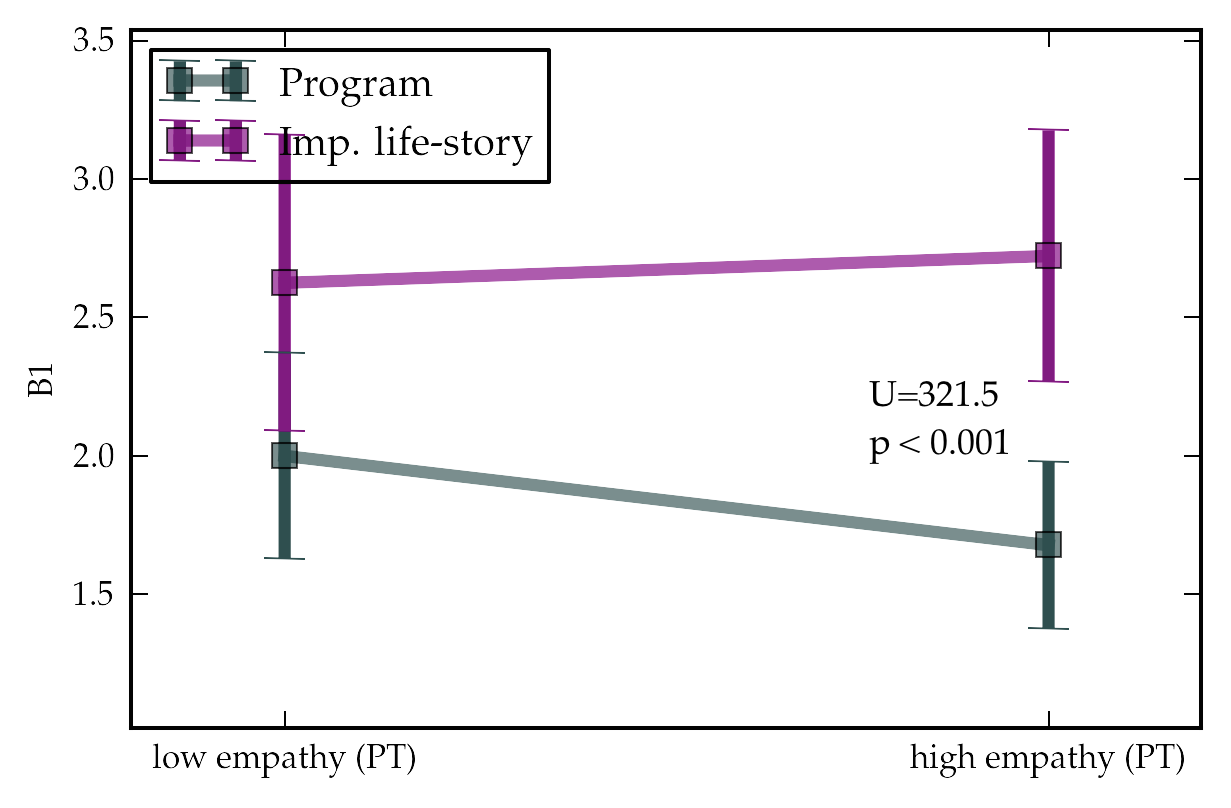
\includegraphics[width=4.6in]{figures/study/rev2/empathy/pt_turk.png}
      \caption{Effect of Perspective Taking (PT) on badness for participants who viewed video (B1) }
      \label{fig_study_pt_turk}
   \end{figure}

   \begin{figure}[thpb]
      \centering
      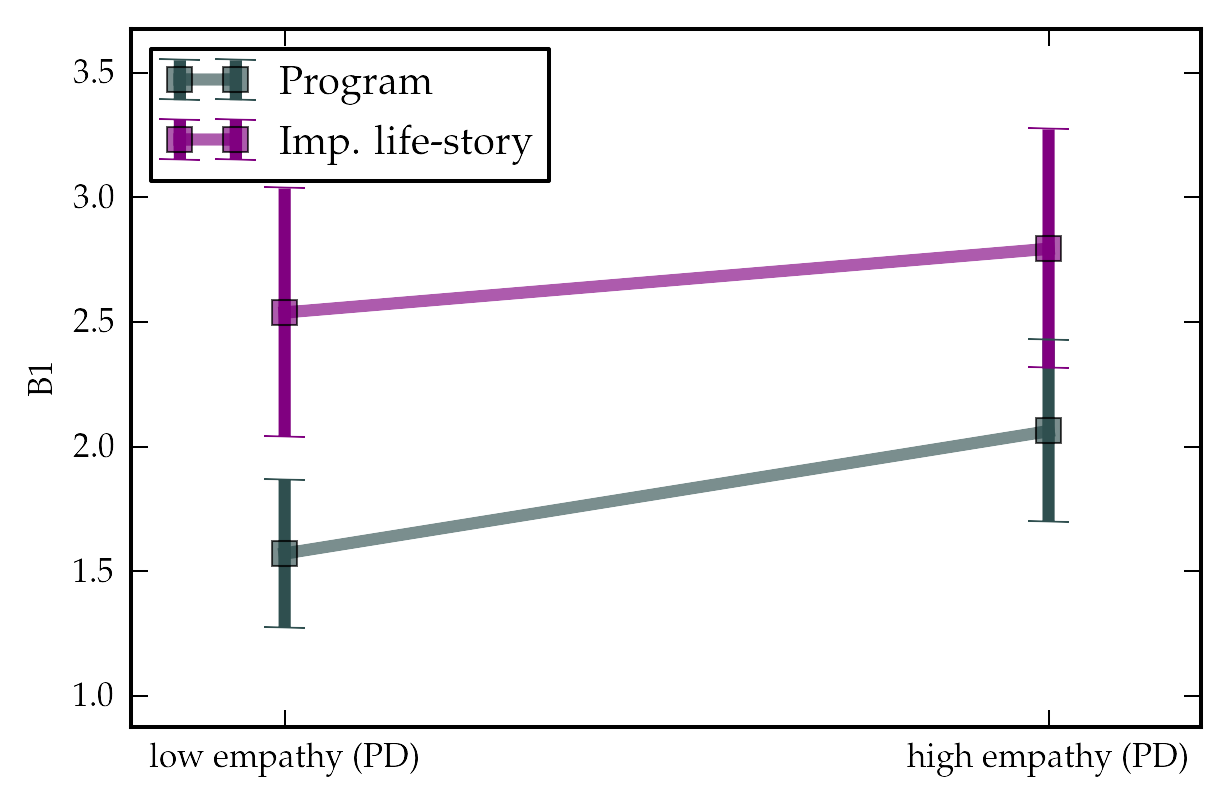
\includegraphics[width=4.6in]{figures/study/rev2/empathy/pd_turk.png}
      \caption{Effect of Personal Distress (PD) on badness for participants who viewed video (B1)}
      \label{fig_study_pd_turk}
   \end{figure}

    \begin{figure}[thpb]
      \centering
      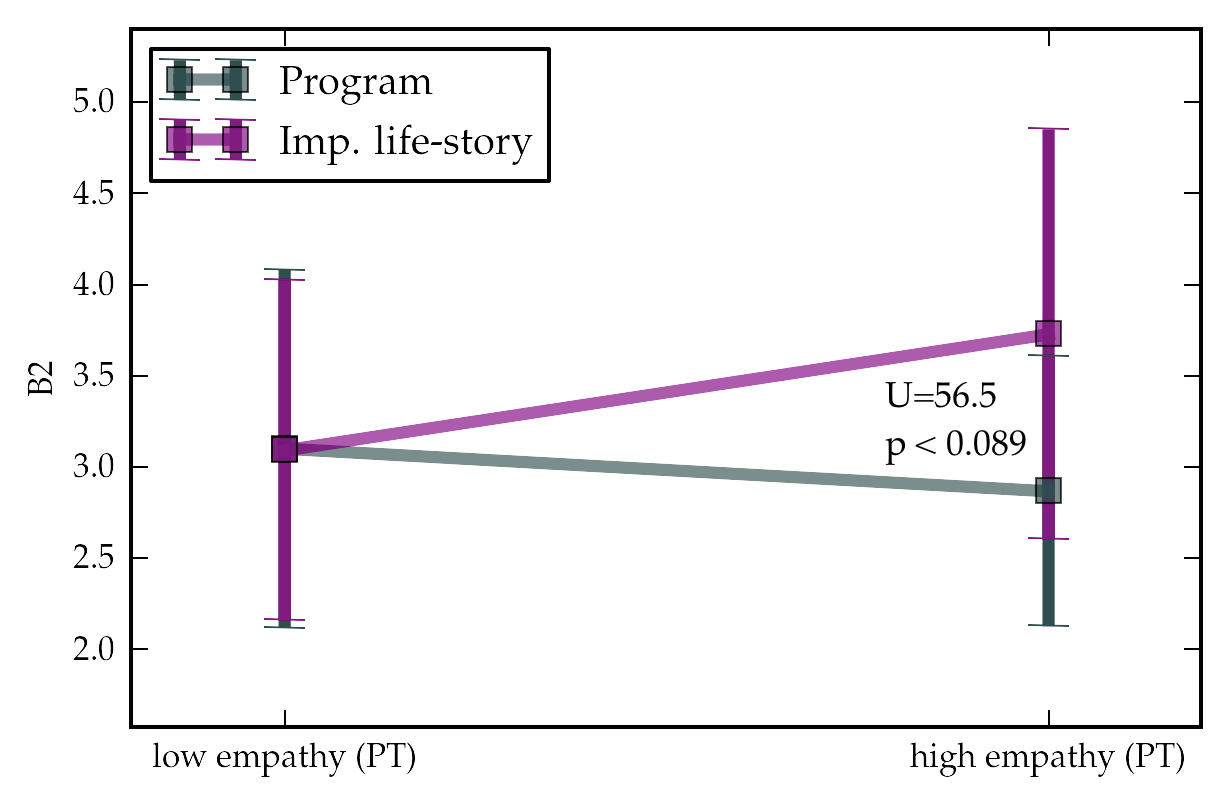
\includegraphics[width=4.6in]{figures/study/rev2/empathy/pt_u.png}
      \caption{Effect of Perspective Taking (PT) on badness for participants who viewed video and interacted but didn't see memory loss (B2)}
      \label{fig_study_pt_u}
   \end{figure}

For participants who interacted with the robot, those with high Perspective Taking (PT)felt worse about the robot (B2) with trending significance (Figure \ref{fig_study_pt_u} ) ($\mu_{imp.\ life-story (High PT)}=3.73, \mu_{program (High PT)}=2.87; U=56.5, p < 0.089$). The difference between the conditions diminished if they witness memory loss of the robot. Other subscales of trait empathy do not show significant differences for the interaction subjects. 



\subsection{Impressions of the Robot}

I had hypothesized that by perceiving a story of growth from experience in the implicit life-story condition, subjects would consider that robot to be more animate and anthropomorphic than the programmed robot (H2). Analysis of the Godspeed Questionnaire shows that subjects found the implicit life-story robot to be more animate than the programmed robot ($\mu_{imp.\ life-story}=3.09, \mu_{program}=2.42; U=2121.0, p < 0.001$). Figure \ref{fig_study_animacy} shows perception of animacy for video, and video with interaction cases across two conditions. Perception of animacy increases with physical interaction for both conditions. Similar pattern holds for anthropomorphic perception, likeability and impression of intelligence (Figures \ref{fig_study_anthropomorphic}, \ref{fig_study_likeability}, \ref{fig_study_intelligence}.) Anthropomorphic shows significant and the greatest difference after the video manipulation. Again, perceived anthropomorphism increases but the difference between the conditions loses significance in the interaction scenario. The data is summarized in table \ref{table_godspeed}.

\begin{table}
\renewcommand{\arraystretch}{1.3}
\caption{Impressions of the robot on the Godspeed Questionnaire}
\label{table_godspeed}
\centering
\begin{tabular}{c|c||c|c|c}
\hline
Godspeed & Interact & Program & Life-story & Mann-Whitney U, p\\
\hline\hline
Animacy & No & 2.26 & 2.96  & \specialcell{$U=1002$\\,$p<0.001**$} \\
\hline
Animacy & Yes & 2.82 & 3.42 & \specialcell{$U=184.5$\\,$p<0.027*$} \\
\hline
Anthrop. & No & 1.64 & 2.45 &  \specialcell{$U=937$\\,$p<0.001**$} \\
\hline
Anthrop. & Yes & 2.51 & 3.02 & \specialcell{$U=220.0$\\,$p<0.122$} \\
\hline
Likeability & No & 3.33 & 3.90 & \specialcell{$U=917$\\,$p<0.001**$} \\
\hline
Likeability & Yes & 3.86 & 4.31 & \specialcell{$U=185.5$\\,$p<0.028*$} \\
\hline
Intelligence & No & 2.60 & 3.16  & \specialcell{$U=1060$\\,$p<0.001**$} \\
\hline
Intelligence & Yes & 2.94 & 3.48 & \specialcell{$U=206$\\,$p<0.072$} \\
\hline
\end{tabular}
\end{table}


   \begin{figure}[thpb]
      \centering
      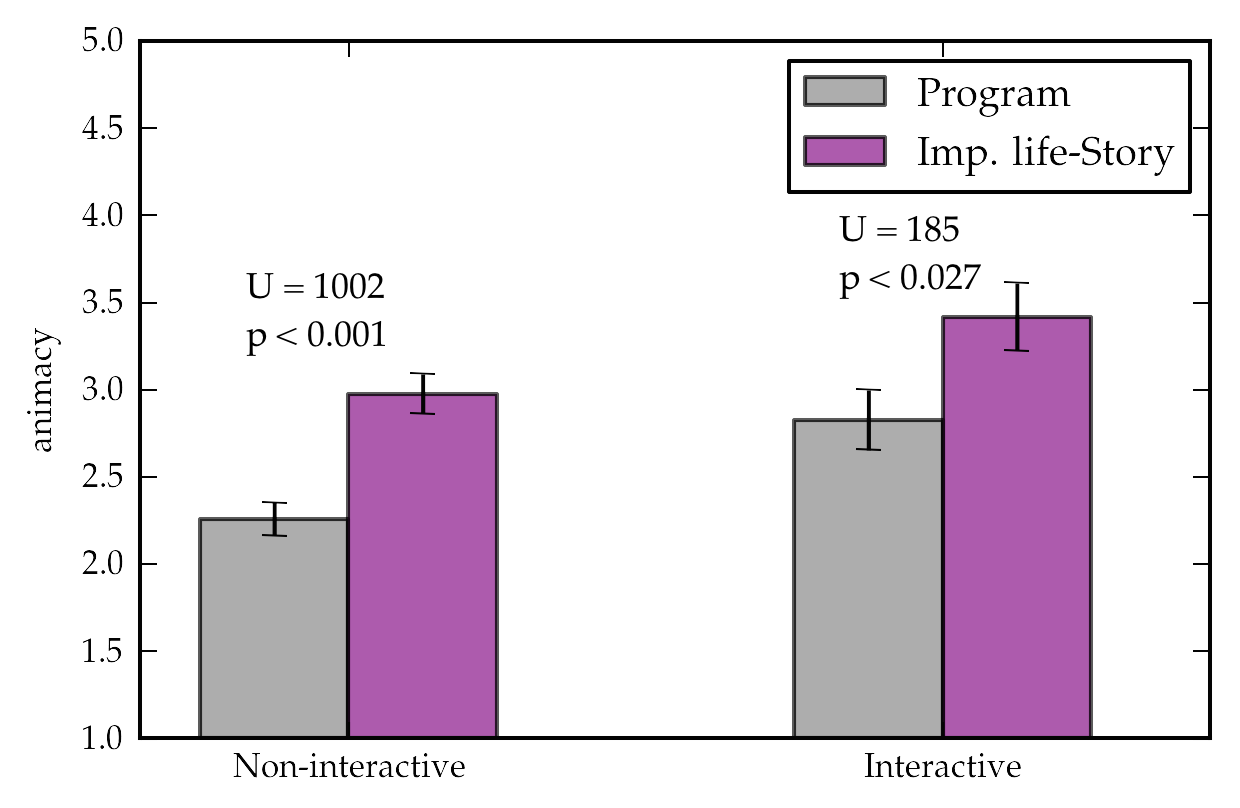
\includegraphics[width=4in]{figures/study/rev2/godspeed/animacy.png}
      \caption{Impression of the robot on the animacy scale. Figure shows significantly greater perception of animacy for implicit life-story condition across video and video with interaction participants}
      \label{fig_study_animacy}
   \end{figure}


   \begin{figure}[thpb]
      \centering
      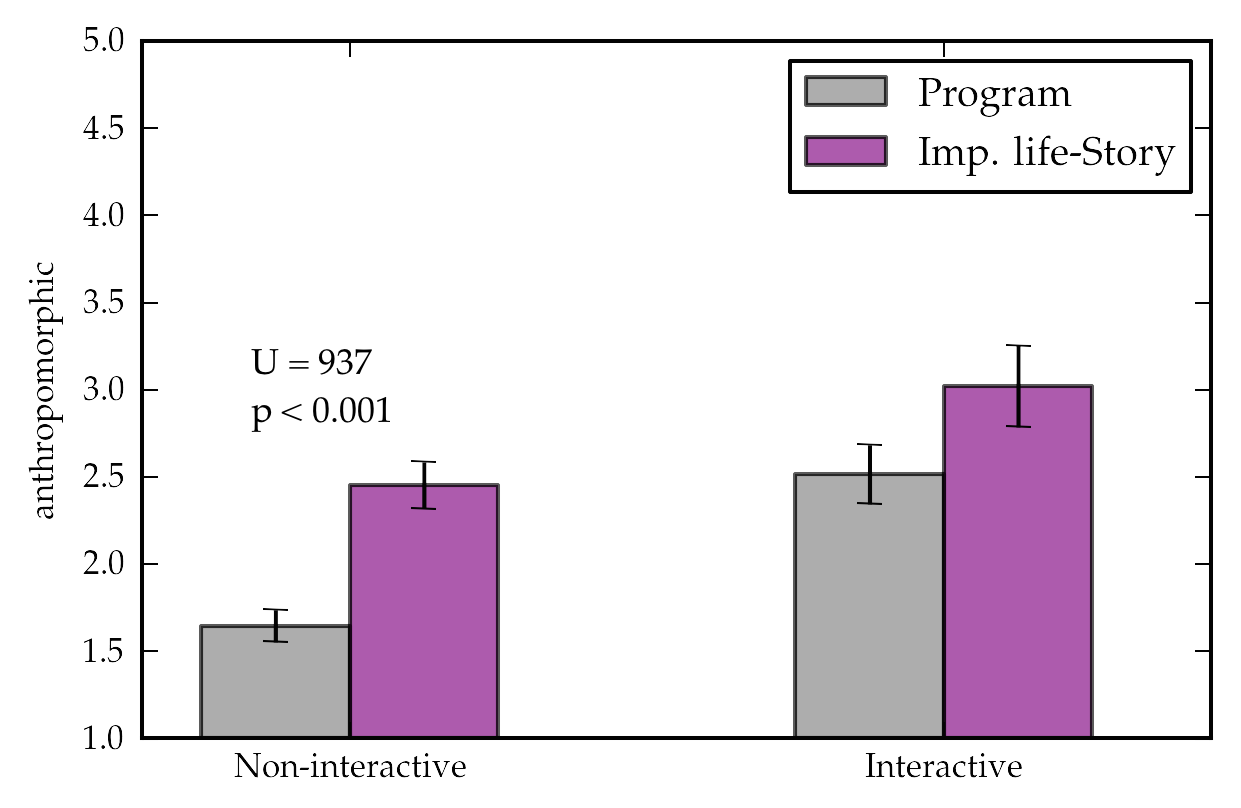
\includegraphics[width=4in]{figures/study/rev2/godspeed/anthropomorphic.png}
      \caption{Impression of the robot on the anthropomorphic scale}
      \label{fig_study_anthropomorphic}
   \end{figure}


   \begin{figure}[thpb]
      \centering
      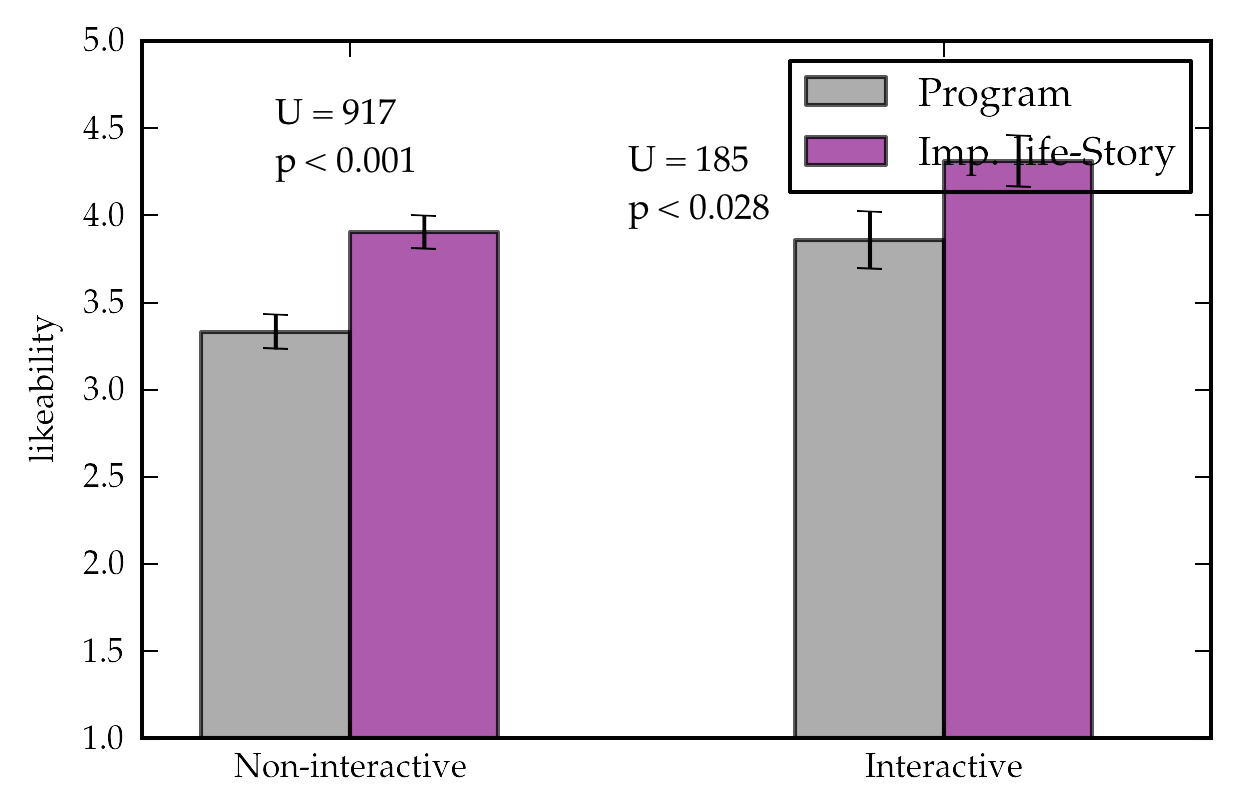
\includegraphics[width=4in]{figures/study/rev2/godspeed/likeability.png}
      \caption{Impression of the robot on the likeability scale}
      \label{fig_study_likeability}
   \end{figure}

   \begin{figure}[thpb]
      \centering
      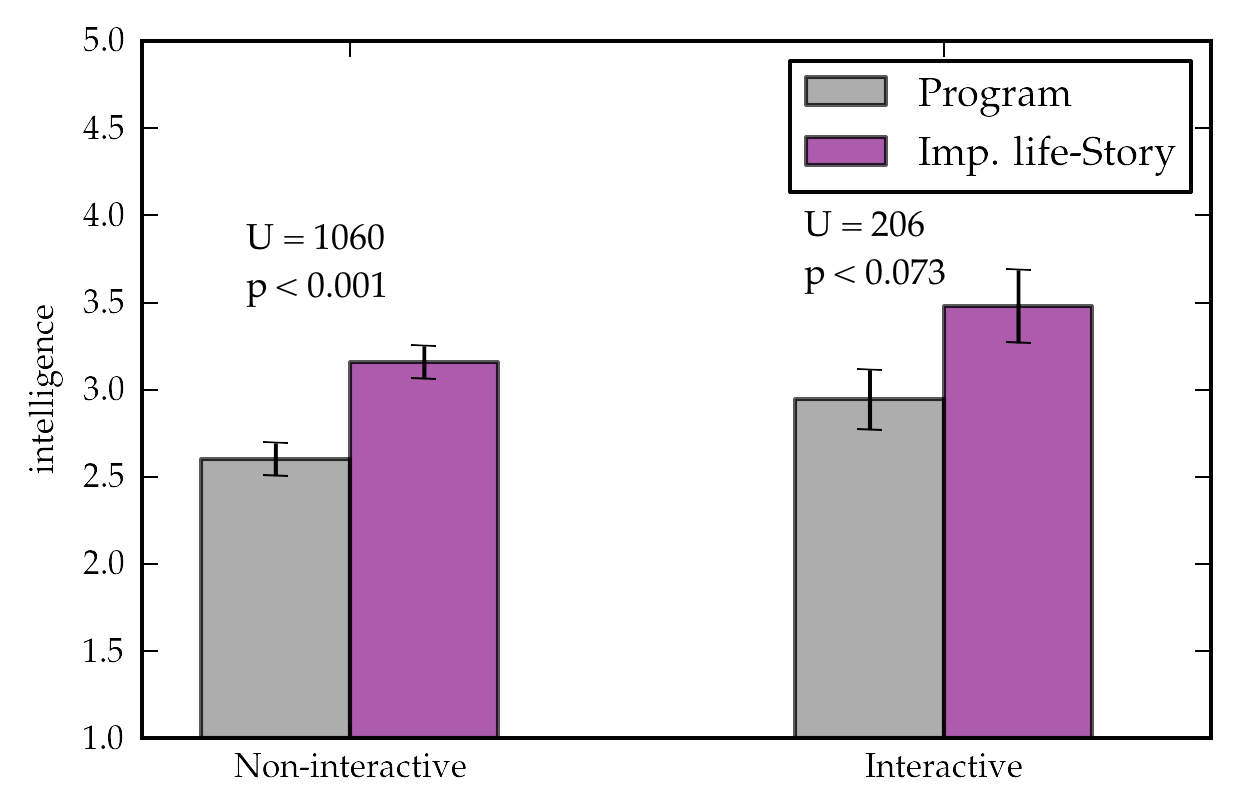
\includegraphics[width=4in]{figures/study/rev2/godspeed/intelligence.png}
      \caption{Impression of the robot on the intelligence scale}
      \label{fig_study_intelligence}
   \end{figure}


Figure \ref{fig_study_godspeed_madness} shows the rating of the robot on the individual questions that comprise the Godspeed questionnaire. I note here though that the robot rates low on the Mechanical vs Organic question which factors into animacy subscale. 


   \begin{figure}[thpb]
      \centering
      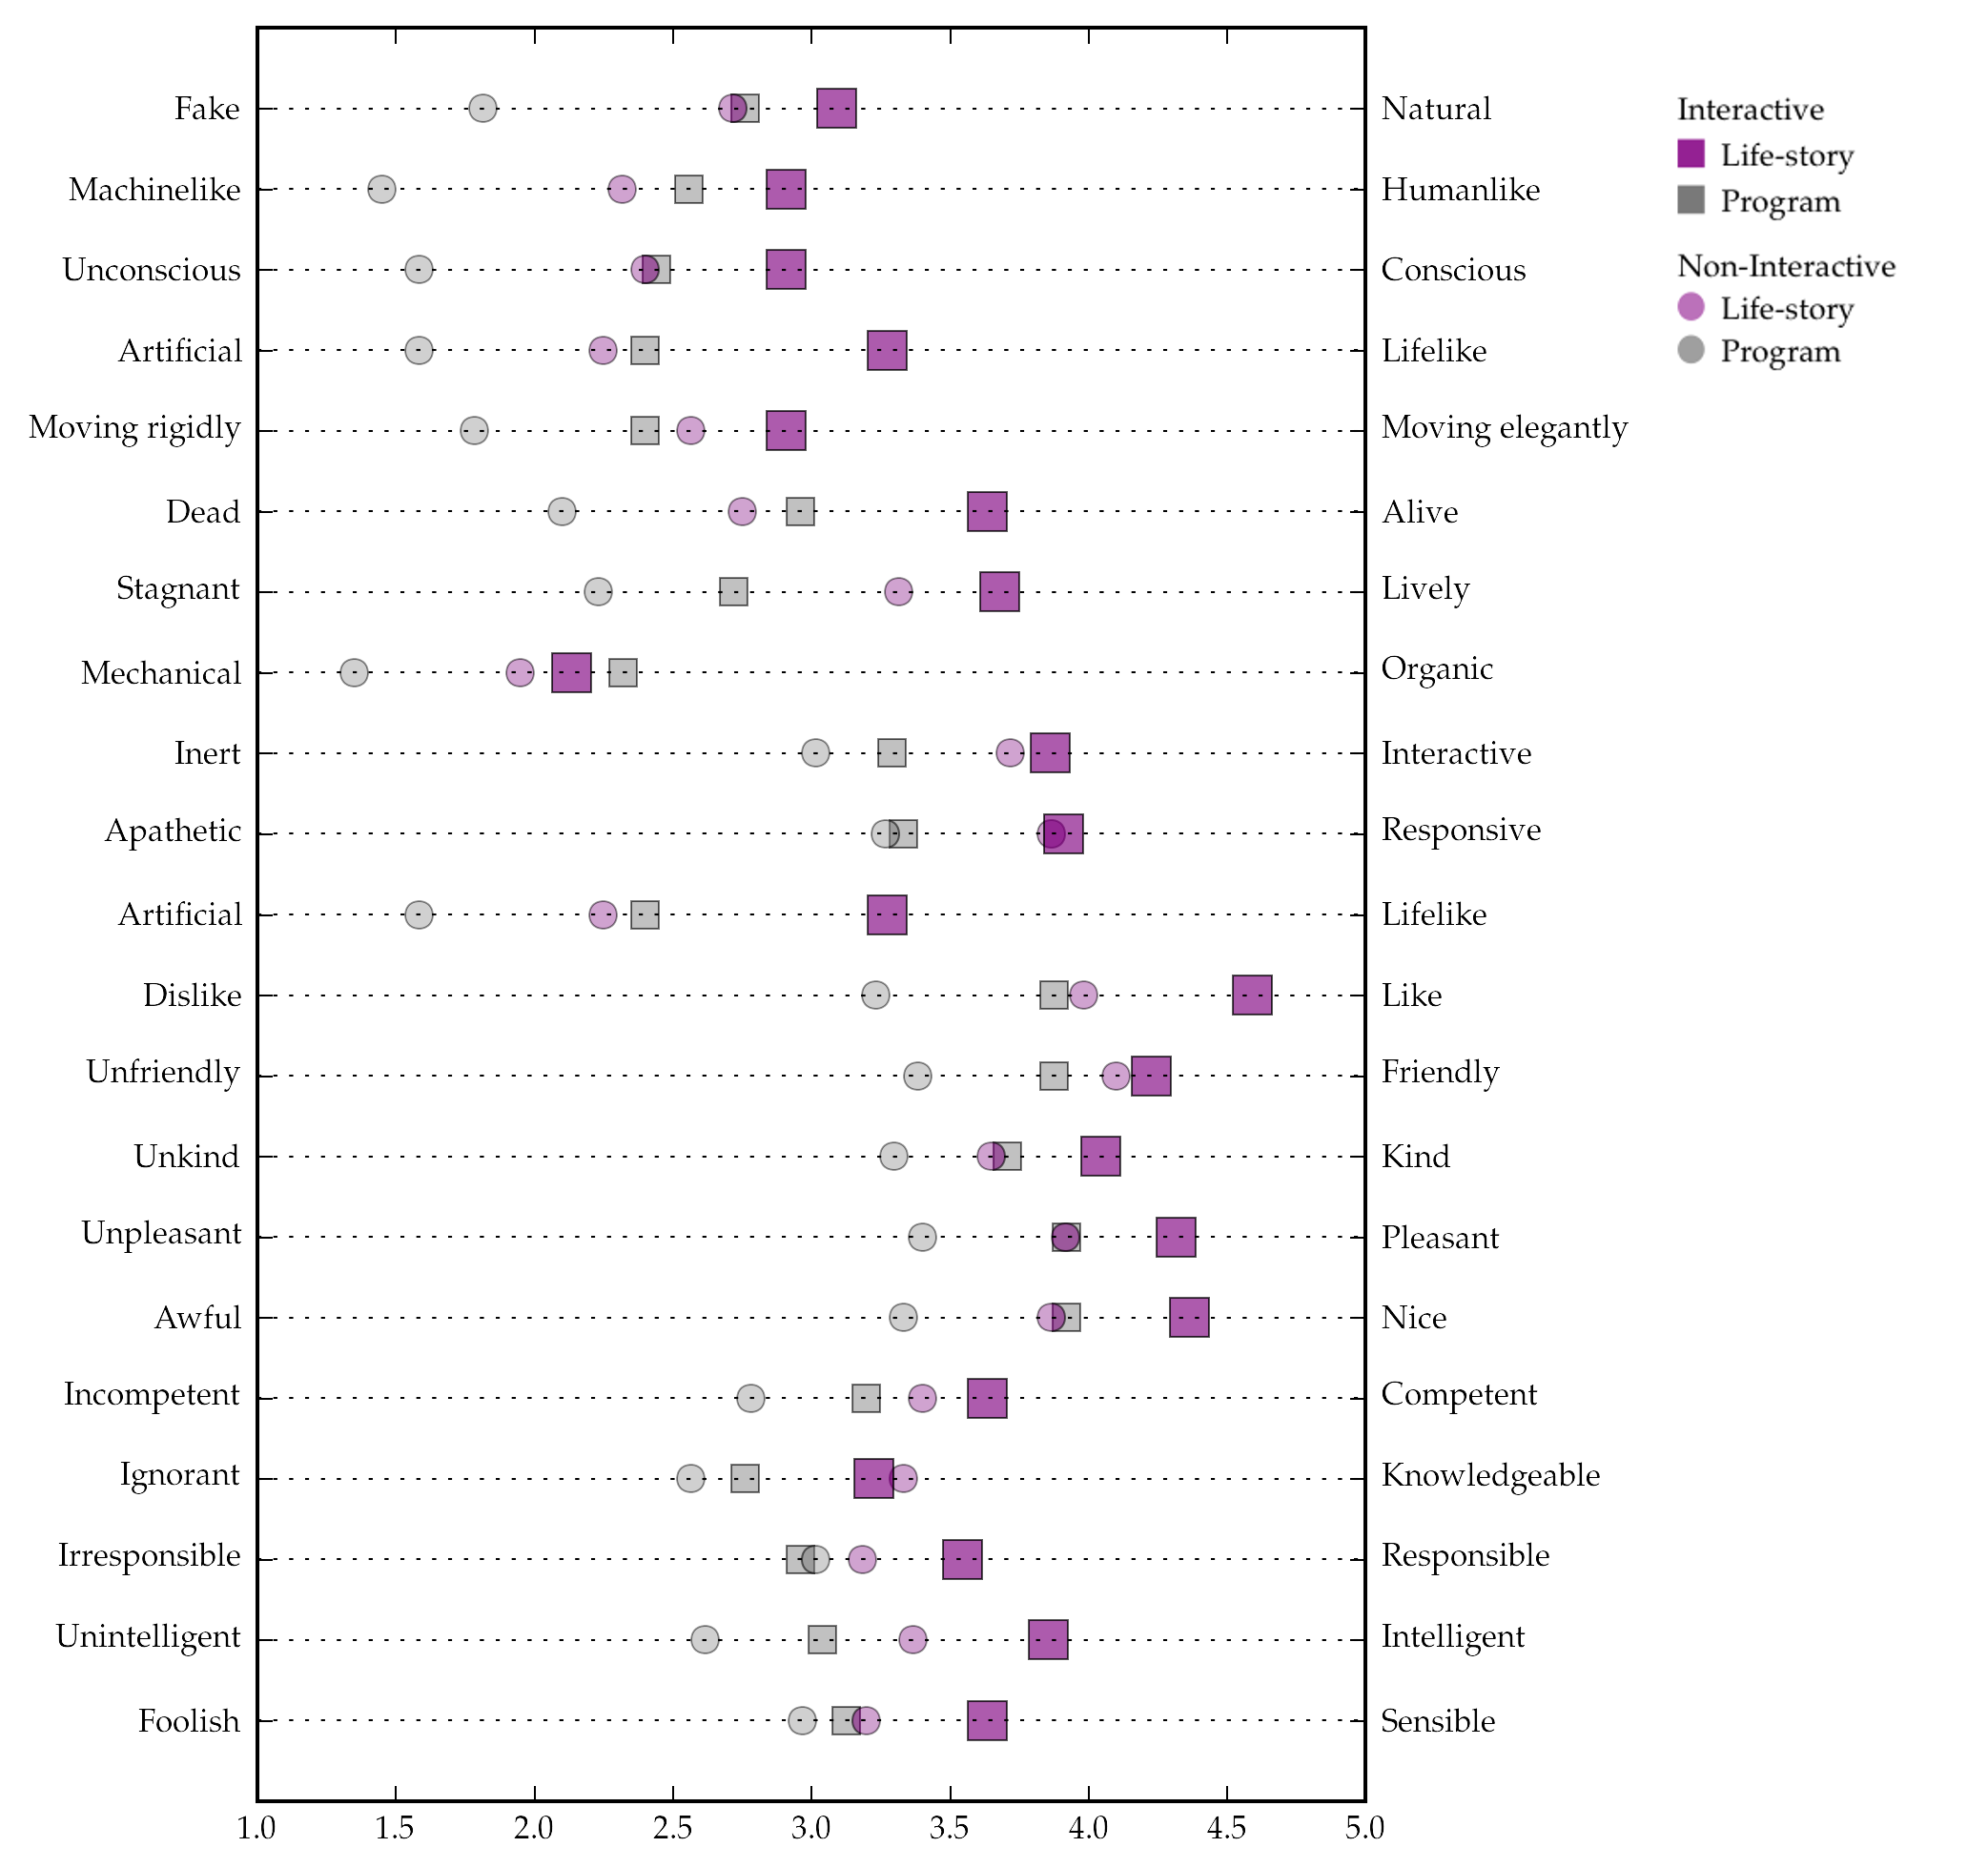
\includegraphics[width=6in]{figures/study/rev2/godspeed/godspeed_madness_legend.png}
      \caption{Impression of the robot on all the godspeed questions. See Appendix \ref{chap_app_godspeed}.}
      \label{fig_study_godspeed_madness}
   \end{figure}


\subsection{Pen Drop}


   \begin{figure}[thpb]
      \centering
      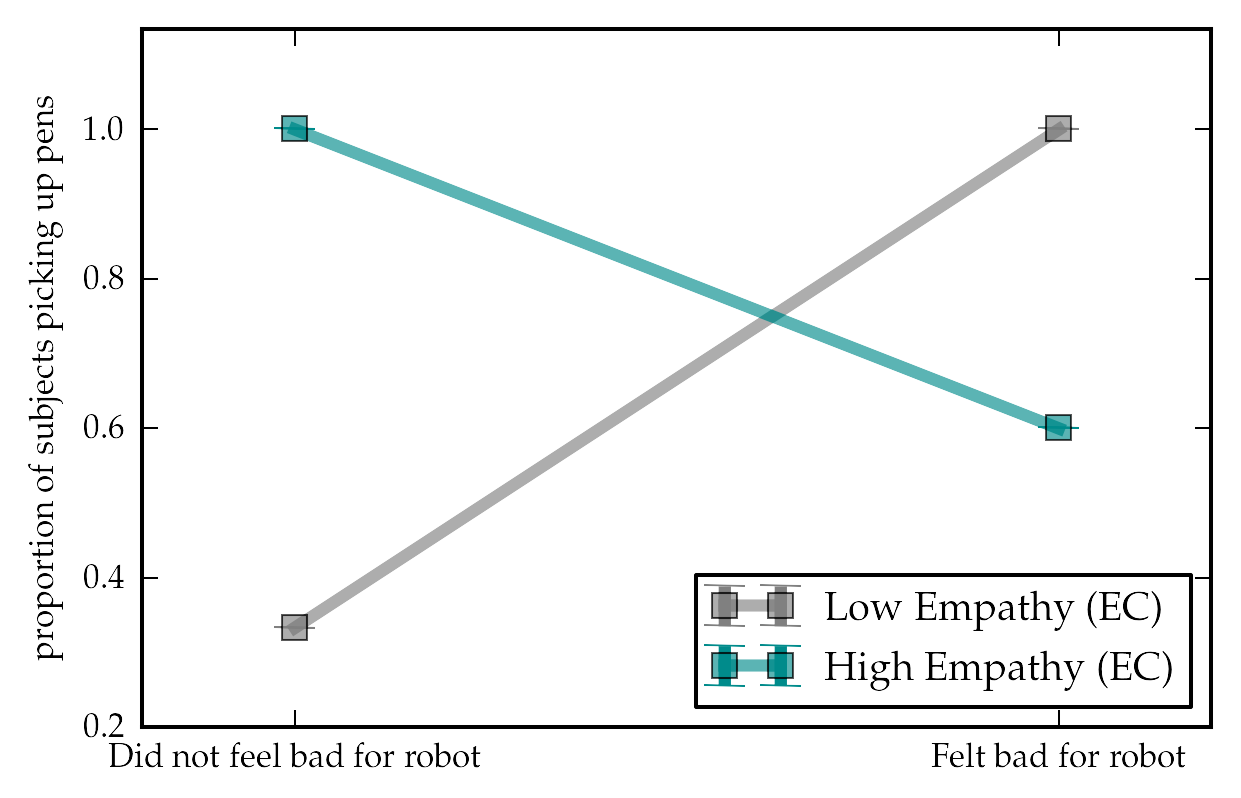
\includegraphics[width=4.6in]{figures/study/rev2/pen/ec_prop.png}
      \caption{Figure showing interaction of feeling bad for the robot (B3) and empathic concern (EC) on propensity to help another pick up dropped pens}
      \label{fig_study_ec_prop}
   \end{figure}


I analyzed the pen pickup data to see if feeling bad about the robot had an effect on subject's inclination to help others (H5). Most subjects picked up the pen ($p=0.71, N=34$). 

Irrespective of the experiment manipulation, I separated the subjects across the median value of self-reported badness (B3) ($median = 4.0$) into two buckets: those who felt bad and those who didn't. As per the empathy analysis in the prior section, I divided the population into high and low empathy buckets across median for each sub-scale of empathy. I calculated the proportion of pen pickups for each of the 4 buckets (empathy $x$ badness levels) per subscale. 

Figure \ref{fig_study_ec_prop} shows the interaction of badness and empathic concern (EC) on proportion of pen pickup. Each bucket had at last 7 subjects. 2-way ANOVA on interaction between pen pickup, empathic concern EC and badness showed the interaction is significant ($F(1,30)=6.453, p < 0.001$). The residuals were normal by Shapiro-Wilks test. If I consider just the individuals with low EC, the change in pickup rate is significant by Fisher's exact test on a 2x2 contigency table (pickup $x$ badness level) ($p < 0.01$). The change for high EC population in proportion of pen pickup is not significant across bucketized badness.

The difference in self-reported badness (B3) between those who picked up pens and those who didn't is significant for both high and low EC. For high EC, B3 drops when they pickup pen compared to when they don't ($\mu_{no\ pickup}=5.0, \mu_{pickup}=3.38; U=10.0, p < 0.029$). For low EC, B3 increases when they pickup pen compared to when they don't ($\mu_{no\ pickup}=2.0, \mu_{pickup}=3.91; U=3.0, p < 0.002$).


Other empathy subscales did not show significant interaction. 


%TODO some intro

\section{Discussion}
\subsection{Implicit life-story of robots}

The validation study results showed that people felt worse if a robot with a experience story (the implicit life-story condition) lost its memory compared to a programmed robot (the program condition). There was a wide range of responses to the robot losing its memory. Why asked why they felt bad about the robot's memory loss, subjects in the implicit life-story condition responded that:

\begin{quotation}
BT5: ``It is almost like a child learning.''

BT5: ``The robot seemed to enjoy the people he met.''

BT5: ``The robot started with nothing [and] build those memories, those favorite words. It learned, that was all it knew, its world. ''

BT5: ``I don't know, I mean, humans are just programming after all like a robot too... and I would feel bad too about a human losing all of their memories.''

BI4: ``It felt like the death of a character.''

BT5: ``Because it learned from its experiences and those experiences are unique. They probably can't be experienced again, at least not in the same way.''

BT5: ``I felt connected to the robot.''

BT5: ``Because all those memories will be lost, like tears in rain.''
\end{quotation}

Some participants in the implicit life-story condition were not moved by the prospect of the robot losing it's memory. One noted: ``I do not care about the stupid robot.'' Others suggested that since it was a machine with the capacity for relearning, it could just relearn what it was losing.

Perhaps unsurprisingly, the sentiment that the robot is simply a machine was seen more frequently in the program condition. Subjects said that they didn't feel bad for the robot beacuse ``it is just a robot'' or ``robots don't have emotions or feelings.'' Other responses included:

\begin{quotation}
AT3: ``I mean the robot is very cute so it almost reminds me of Wall-E... so I would feel bad if the robot lost anything but I must need to remember that this robot has no feelings.''

AT1: ``It doesn't really have any consciousness or sentence formation [ability], it just repeats stuff.''

AT1: ``The robot does not really have any personality, it seems very programmed. It does not seem like you are talking to \lq someone\rq, but just a randomized computer program.''

AT1: ``It's a robot. It's not a person.''
\end{quotation}


The themes that emerged for those who felt bad are that they see the robot as life-like, capable of emotions (``enjoy the people he met''), as a product of unique meaningful experiences (``favorite words'') and not unlike themselves (``connected to the robot''). This is in contrast to those in the program condition who thought of the robot more as a machine without capacity for feelings. Over the course of this chapter, I will delve more into these themes in discussion of the quantitative data.

The mention of unique experiences is worth discussing further. The particular test the study used, feeling bad for loss, is meaningless without uniqueness as there would be nothing to be lost otherwise. The robot in both conditions was unique, one where its memories were formed by unique experiences and the other by random selection of words. The data shows that the experience of the implicit life-story matters more for feeling bad for the robot compared to an uniqueness generated by randomness. It could be argued that perhaps the difference in B1 was due to participants not being aware of the uniqueness of the random words in the program condition. To address this, I re-ran the study for non-interactive case with the back-story of the program condition modified to include the following two lines at the end: ``We have programmed many robots with randomly generated memories. However, the unique combination of randomly selected words makes this robot different.'' The implicit life-story condition was left as described earlier. Videos were the same. Even with the modified program condition, the results were similar: subjects felt significantly worse in the implicit life-story condition compared to the program condition ($\mu_{imp.\ life-story}=2.94, \mu_{program}=1.68; N=60; U=219.5, p < 0.001$).

% BT5``After watching the video you feel a small connection to the robot. i would not like it if i lost my memories and the robot seemed to have some good ones so i would feel bad if it did!''




% BT1``It doesn't have conscious and to me it's just a computer.  I wouldn't feel bad if my computer lost it's memory.  It can always relearn again.''

% BT1


% BT5``It almost seemed lifelike.  It reminded me of my african grey parrot, Dante.''


% BT5``Because all those memories will be lost, like tears in rain. I mean it took a lot of effort from many different people to get the robot this far. It seems like such a waste to destroy all that work. Plus the robot reminds me of a real pet with it behavior. I can imagine people getting attached to it and might feel bad as a result.''

% BT1``it does not have a conscience, i would feel bad for the makers''

% 

% BT1``It's not my robot?''

\subsection{Differences between interaction and non-interaction}

The study also showed that across conditions, people felt worse after interacting with the robot and seeings its memory loss (B3 vs. B1) or (B2 vs. B1). However, the difference in B3 between the conditions decreased. One explanation for this decrease in difference is that physical interaction with the robot is contributing to empathy and masking the effect of the manipulation. In particular, the distress of the robot at memory erasure seemed to affect participants irrespective of the condition.  As described in the last chapter, when the robot's memory was erased it thrashed around making distressed sounds. Afterwards it tilted its head forward and became silent briefly. One participant from the program condition explained why they felt bad for the robot: ``The robot started jerking around almost like it was having a seizure. It was not unlike a human being being hurt in some way.'' Another participant, also in the program condition, felt bad because: ``robot looked and acted sad.'' 

These results mirror what I saw in the hexbug study where movement mitigated the effect of story manipulation (Section \ref{sec_hexbug_discussion} ). In that study, movement made people less hesitant to harm the robot, presumably due to the insect like motion of the hexbug. Based on prior work on robots with human stories \cite{gockley_valerie_roboreceptionist}, I speculate that once the novelty of physical interaction with a robot has worn off, the effect due to implicit life stories will be salient again, particularly if the robot continues to change over time. I will revisit this idea when I talk about potential future work.


\subsection{Empathy for the robot}


Empathy is the quality of feeling what others feel. So if people feel worse when an implicit life-story robot is being harmed then it suggests that they feel empathy for it. In the earlier study, people empathized more with the hexbug, and were more reluctant to harm it, when it was given an implicit life-story. Empathy was similarly demonstrated by subjects' responses in the sound robot study. When asked why they felt bad, one subject, in the implicit life-story condition, said: ``After watching the video you feel a small connection to the robot. i would not like it if i lost my memories and the robot seemed to have some good ones so i would feel bad if it did!''

Just as in the hexbug study, my results in this study showed that across conditions, those with higher level of trait empathic concern (EC) felt worse (B3) about a robot being harmed compared to those with low EC. This further supports the argument that empathy had a role in people feeling bad for the robot, rather than their reaction just being due to destruction of value. 

%TODO reference someone else

When I examine B1 (how bad the subjects felt just after they watched the videos), the effect of the story manipulation was more pronounced on those with high trait empathy. This suggests that the implicit life-story engenders empathy. While this result is similar to what we obtained in the hexbug study, in this study, in addition to empathic concern (EC), high level of fantasy (FS) and perspective taking (PT) trait empathies also significantly increased effect of stories on badness (B1) with the difference being greatest for FS. FS, to quote Davis ``taps respondents' tendencies to transpose themselves imaginatively into the feelings and actions of fictitious characters in books, movies, and plays,'' while PT is defined as ``the tendency to spontaneously adopt the psychological point of view of others'' \cite{davis_multidimensional_empathy}. When I had laid out my argument for why implicit life-stories could cause empathy, I had suggested that the mechanism at work might be that seeing a robot's experience ambiguously told through changes, engages us in imagining ourselves in its place, and we use our own experience to reconstruct its experience. The effects of FS and PT trait empathies on badness (B1) seen in the study are consistent with this hypothesized mechanism. 

Rosenthal-von der P{\"u}tten et al. found a correlation between subjects' FS scores and their responses to the robots being mistreated on video \cite{rosenthal_emotional_reaction}. However, across conditions, I did not find a significant difference in badness (B1) for subjects with high FS compared to those with low FS. Rather the data shows, for those with high FS, there is a significant difference in B1 between implicit life-story and program. This suggests that effect I am seeing is not peculiar to video based empathy induction, but is related to the story manipulation. 


\subsection{Effect on empathy for others}

I had hypothesized that empathy for a robot would have an impact on empathy for another person. This study's data showed that if observing the robot suffering harm had no impact on how bad subjects felt (B3), then high trait empathic concern (EC) subjects would help another person, while low EC subjects would be less likely to. This behavior is consistent with the definition of empathic concern. 

However, the data showed if low EC individuals \emph{were} affected by the robot and felt bad, they would subsequently be more likely to help another in distress. This result is consistent with a study by Barnett et al. that found that subjects when given an empathy arousing stimulus, for instance seeing video of crippled children suffering, would transfer the empathy to an unrelated target group and show pro-social behavior towards the target \cite{barnett_empathy_transfer}. 
A counterintuitive result from this study is that high EC individuals were less likely to help another person if they felt bad for the robot compared when they didn't feel bad.  In human-human interactions, the act of being empathic is known to reduce the capacity for empathy afterwards \cite{figley_compassion_fatigue_therapists}. It could be that I observed a similar effect in human-robot interaction for high empathic individuals. 

%Empathic reaction to another's suffering has been known to lead to compassion fatigue in human-human interactions where the empathizer has reduced capacity for empathy afterwards  
%% pen pickup

\subsection{Participant's impressions of the robot}

Participant's perceptions of the robot on the measures of animacy, anthropomorphism, likeability and intelligence were higher in the implicit life-story condition than in the program condition. 

In the implicit life-story condition, participants often compared the robot to a pet: ``It almost seemed lifelike.  It reminded me of my African grey parrot, Dante.'' While perceived experience made the robot seem more life-like and alive (see Figure \ref{fig_study_godspeed_madness}), overall the robot was considered to be mechanical rather than organic. The seeming contradiction of seeing the robot as ``alive'' yet ``mechanical'' could be explained by the form of the robot. The design prominently featured a speaker for a face and exposed the internal workings.

Participant's perceptions of the robot relating to its ``likeability'' were somewhat unexpected. While implicit life-story did improve likeability, in both conditions subjects considered the robot to be ``kind'', ``nice'', ``pleasant'' and ``friendly'' (Figure \ref{fig_study_godspeed_madness}). I suggest that the rounded and juvenile form of the robot and its gentle breathing motion may have contributed to the positive perception here. Moreover, the robot does not drive interaction; it speaks when spoken to and if it does speak while overhearing a conversation, it doesn't require attention.

%TODO explain why the passive behavior contributes

Participant's perceiving the robot as more intelligence when they were shown its life story could be due to the common association between ``intelligence'' and ``learning'', so that when presented with evidence that the robot had the ability to learn subjects saw it as more intelligent than when they were told that it was simply following a program - particularly when that program was explained to them.

Often, participants stayed after the experiment to talk with the experimenter about what they thought of the robot. Some subjects said that they talk to themselves when they were alone and thought that the robot would make a good listening companion. A few mentioned that they would want to watch TV with the robot and have the robot comment in or share the experience with them. Not all reactions were positive though: one subject was uncomfortable with the idea of a robot that could be listening to what they were saying and said that they would not want to have such a robot at home. However, in general there was interest in the idea of a sound robot as a companion. 


\section{Wrapping up}

I found, in support of my thesis, that people have greater empathy for a robot when it has an implicit life-story.  People also found the robot with implicit life-story to be more animate, anthropomorphic, likable and intelligent. Lastly, I found that empathy for robots can have an effect on empathy for people. 




% 4-21 work
% 4-21 home

